% *******************************************************************************
% * Copyright (c) 2007 by Elexis
% * All rights reserved. This document and the accompanying materials
% * are made available under the terms of the Eclipse Public License v1.0
% * which accompanies this distribution, and is available at
% * http://www.eclipse.org/legal/epl-v10.html
% *
% * Contributors:
% *    G. Weirich
% *
% *  $Id: elexis-notes.tex 4854 2008-12-25 07:41:42Z rgw_ch $
% *******************************************************************************

\documentclass[a4paper]{scrartcl}
\usepackage{german}
\usepackage[utf8]{inputenc}
\usepackage{makeidx}
\makeindex
% Hier ein etwas skurriler Block, der dazu dient, die Unterschiede
% zwischen pdflatex und latex auszubügeln
% Grafiken müssen als png oder gif (für pdflatex) und als eps (für Latex)
% vorhanden sein. Die Endung kann man beim \includegraphics jeweils weglassen,
% das System nimmt je nach Renderer die geeignete Variante.

\newif\ifpdf
\ifx\pdfoutput\undefined
	\pdffalse              	%normales LaTeX wird ausgeführt
\else
	\pdfoutput=1
	\pdftrue               	%pdfLaTeX wird ausgeführt
\fi

\ifpdf
	\usepackage[pdftex]{graphicx}
	\DeclareGraphicsExtensions{.pdf,.jpg,.png}
\else
	\usepackage[dvips]{graphicx}
	\DeclareGraphicsExtensions{.eps}
\fi

\usepackage{floatflt}
\usepackage{wrapfig}
\usepackage[]{hyperref}
\usepackage{color}
\begin{document}
\title{Elexis-Notes}
\author{Gerry Weirich}
\maketitle

\section{Einführung}
Dieses Plugin dient dazu, beliebige nicht-patientenbezogene Informationen und Dokumente abzulegen. Diese können nach beliebigen Kriterien strukturiert und mit Stichwörtern versehen werden.

Ausserdem können, falls in Elexis ein Scanservice\footnote{Ein Scanservice liefert die Fähigkeit, Scanner anzusteuern und kann von einem anderen, separat zu besorgenden Plugin beigesteuert werden, z.b. Omnivore-direct ist ein solcher Service-Provider} vorhanden ist, Dokumente direkt eingescannt werden.

\medskip

elexis-notes benötigt Elexis ab Version 1.4

\section{Installation, Deinstallation, Konfiguration}
Wie üblich wird das Plugin durch einfaches Kopieren ins Plugins-Verzeichnis installiert und durch Löschen aus diesem Verzeichnis wieder deinstalliert.

\begin{figure}
  % Requires \usepackage{graphicx}
  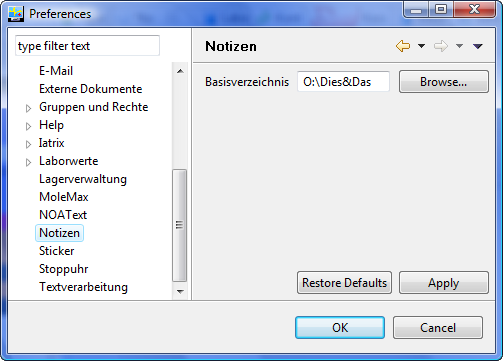
\includegraphics{config}\\
  \caption{Konfiguration}\label{fig:notes1}
\end{figure}

Die Konfiguration (Vgl. Abb. \ref{fig:notes1}) beschränkt sich darauf, ein Basisverzeichnis anzugeben, unterhalb dem  \textit{Elexis-Notes} externe Dokumente ablegen soll.

\section {Verwendung}


\end{document} 